\section{Approach}
\label{sec:method}

This section introduces our solution for \textit{"how to perform type-transition-aware type error detection"}.

\subsection{Overview}

\begin{figure}[!htbp]
\centering
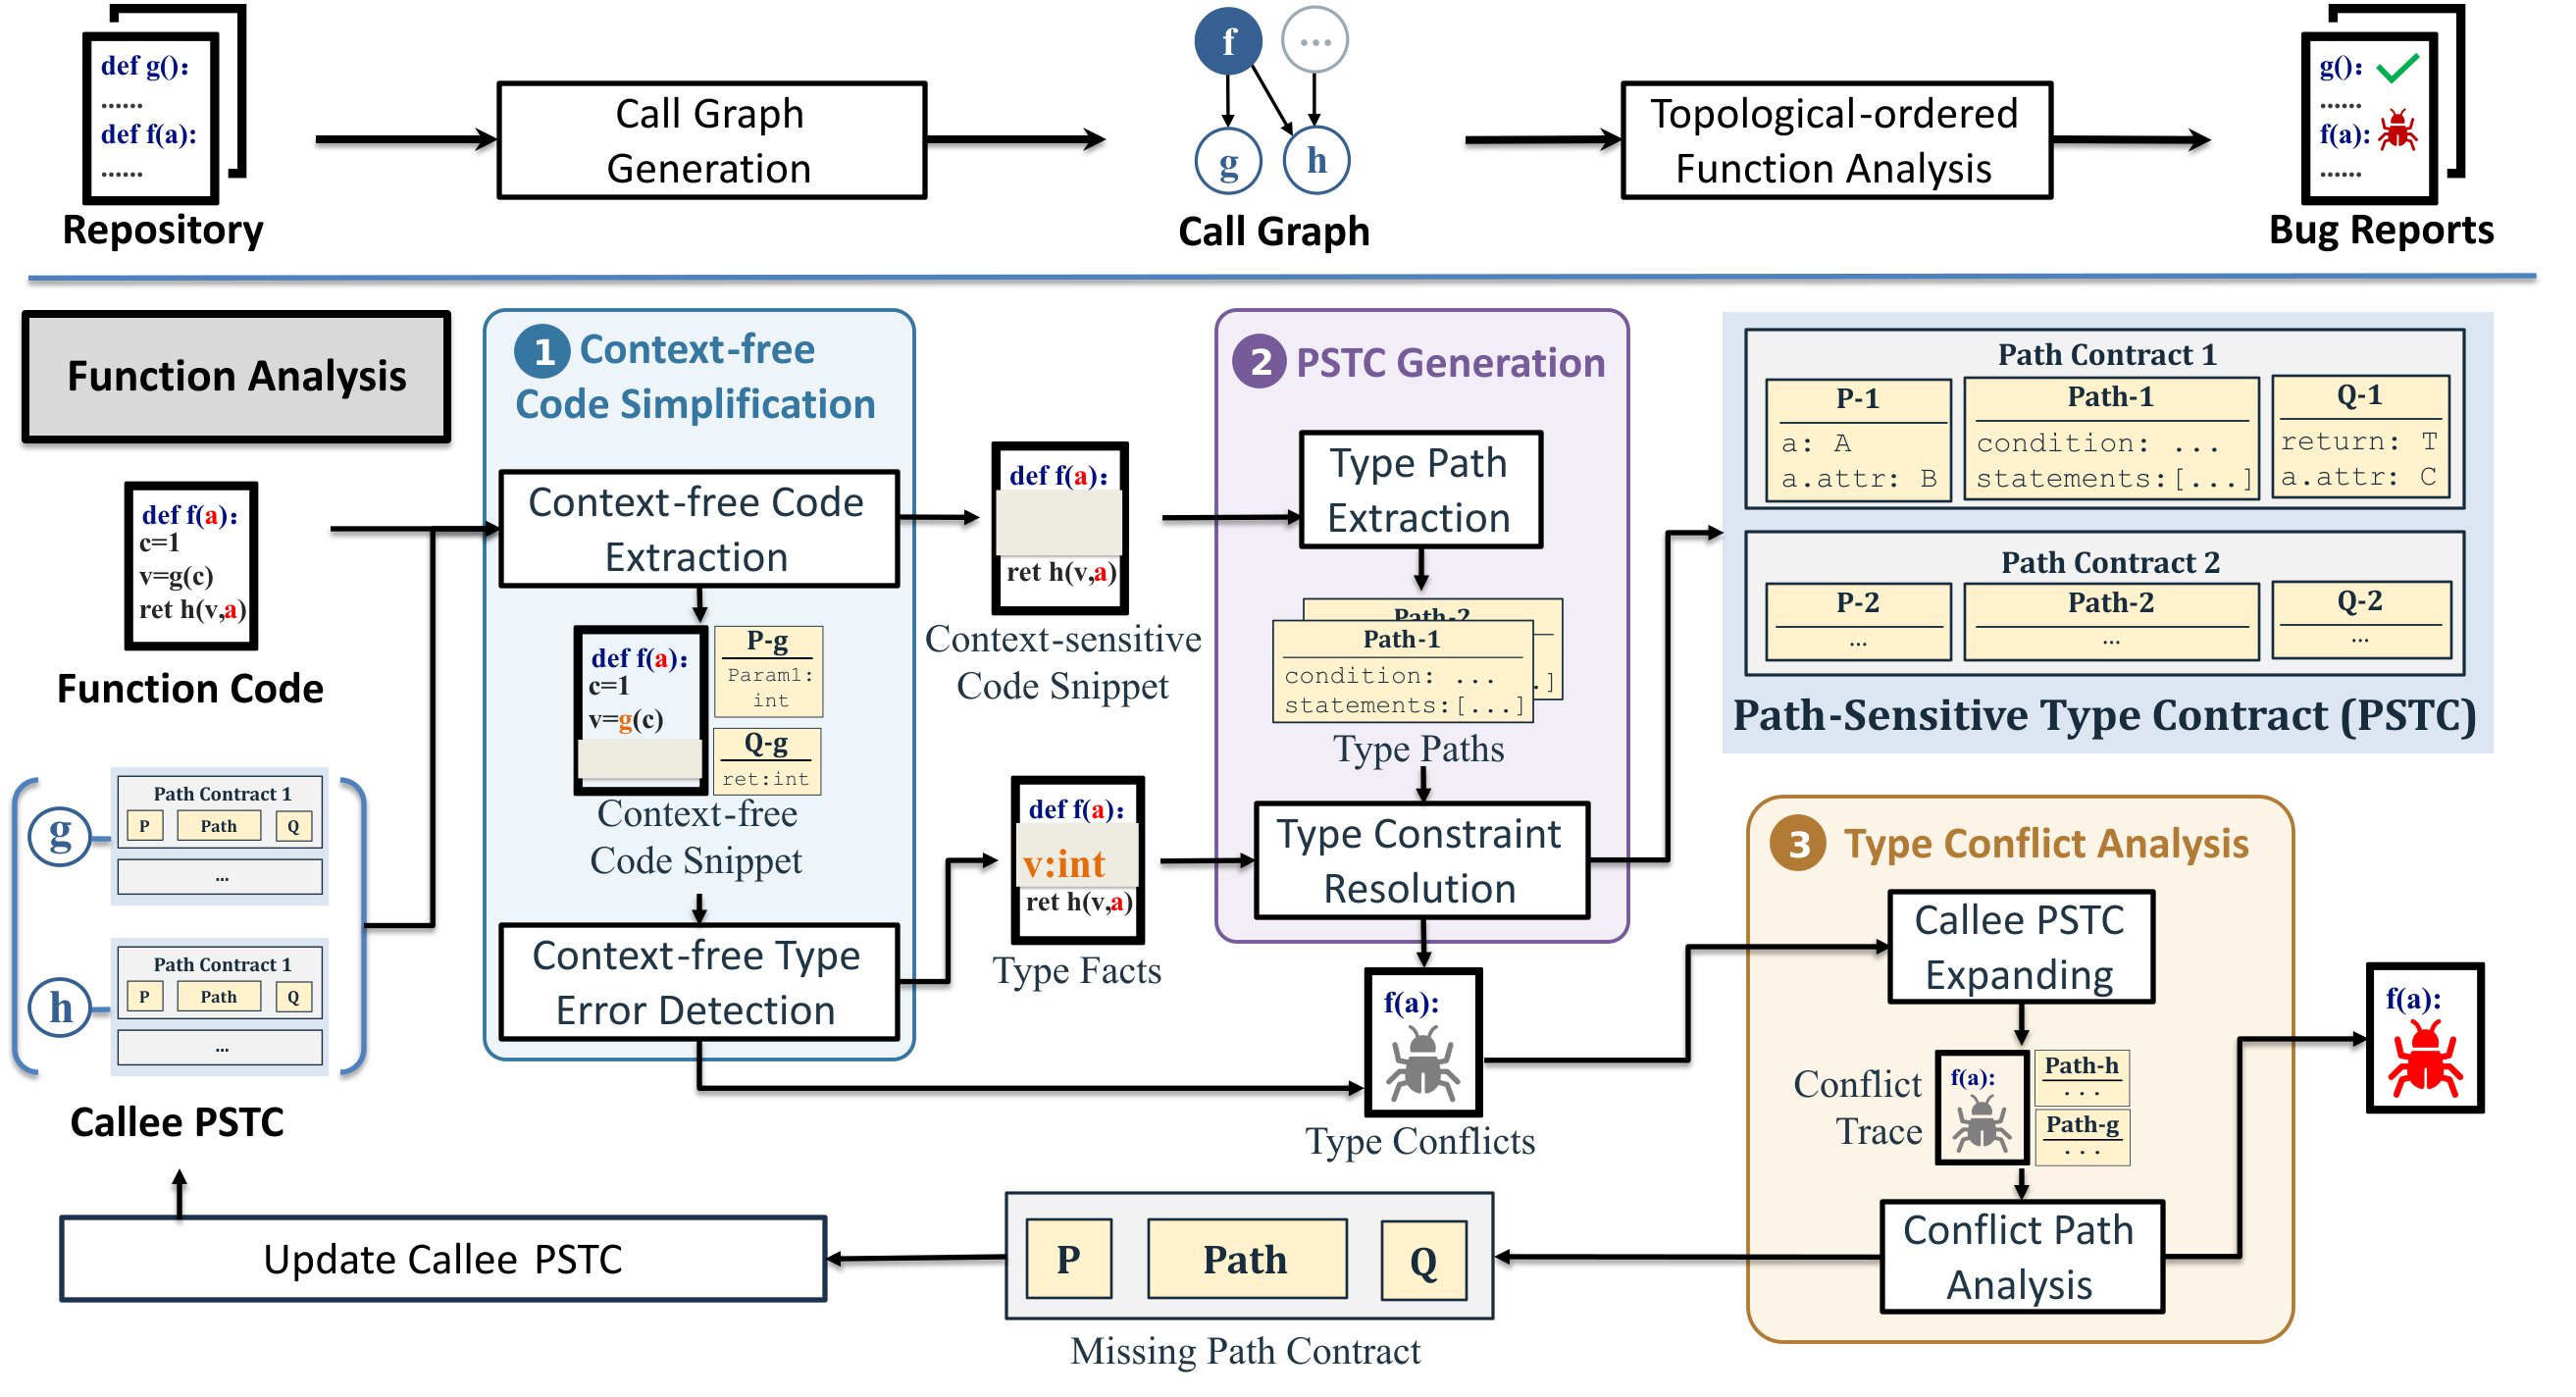
\includegraphics[width=\linewidth]{photos/methodOverview.png}
\caption{Overview of PyTT's workflow}
\label{fig:method-overview}
\end{figure}


Figure~\ref{fig:method-overview} illustrates the workflow of PyTT for type-transition-aware type error detection. 
PyTT processes functions in a callee-before-caller topological order over the call graph. 
For each function, it detects type errors within the function and constructs a 
\emph{path-sensitive type contract} (PSTC) that summarizes the function's type transitions along different execution paths. 
The resulting PSTC is propagated to callers to support interprocedural analysis. 
Specifically, PyTT analyzes each function in three phases.

\textbf{(1) Context-free Code Simplification}. 
To check the uses of variables with known types and prune unnecessary paths, PyTT performs type checking and simplification on code whose type behavior is independent of the function's inputs.
PyTT identifies variables whose types are independent of the function's inputs and uses static analysis to trace their propagation, thereby extracting the context-free code.
It then leverages an LLM to check whether these variables are used correctly and simplifies the extracted code into type information for expressions used in the context-sensitive code, supporting subsequent analysis of that code.

\textbf{(2) PSTC Generation}.
In this phase, PyTT analyzes the remaining context-sensitive code to construct a PSTC that captures the function's type transitions under different execution conditions.
PyTT first identifies explicit execution paths within the context-sensitive code through static analysis.
For each explicit path, PyTT uses an LLM to derive behavioral constraints on the inputs and infer the possible input type-states that satisfy these constraints, thereby identifying distinct implicit paths.
Each path, together with its input and output type-states, forms a path contract, and these contracts collectively constitute the function's PSTC.
Additionally, behavioral constraints that admit no valid input type-state indicate conflicting requirements on the behavior of the variables and are also identified as type errors.

\textbf{(3) Type Conflict Analysis}.
To distinguish type errors from false alarms caused by inaccurate PSTCs, 
PyTT examines the source behavior underlying each detected type conflict.
Once a type conflict is detected, PyTT uses the path recorded in the callee's PSTC 
to trace the conflicting type facts through the relevant caller and callee code.
The type transitions along the resulting interprocedural path are re-inferred using an LLM.
If this analysis confirms a type error, PyTT reports it together with the confirmed interprocedural trace that triggers the error.
Otherwise, the analysis reveals an inaccurate PSTC, which PyTT corrects to dismiss the resulting false alarm.

Following a callee-before-caller topological order over the call graph, 
PyTT first simplifies each function into a context-sensitive code 
snippet in the \textit{Context-free Code Simplification} phase.
The \textit{PSTC Generation} phase then summarizes the type 
transitions along different paths into a PSTC, 
providing interprocedural type-transition information for type error detection in callers.
The PSTC is corrected and updated through the \textit{Type Conflict Analysis} phase.
Once all functions in the repository have been analyzed along the call chains, 
PyTT collects all detected type errors and compiles them into an error report for the repository.

\subsection{Design of Path-Sensitive Type Contracts}
\label{sec:state-model}


The motivating example establishes two requirements for a function
summary. It must describe the change of type to values shared with the caller, and
it must retain the conditions under which each change occurs. 
PyTT therefore needs a summary that connects the incoming type-state and
execution conditions to the types established by the call.

Before defining the contract, we introduce the abstraction that it
relates. 
A \emph{type-state} is a simplified form of program state. It
abstracts away from the concrete values that a program manipulates and
retains only the type information required by the checks of subsequent
operations. At a program point, a type-state describes the type of a
parameter, a local or global variable, or a class or instance attribute.
At point~1 of Figure~\ref{fig:motivating-example}, for example, the
type-state records that the message body holds a string. Because a
function can be called under different type-states, PyTT describes its
behavior as a relation between the type-states at its entry and its exit,
rather than in terms of particular values.


  \begin{definition}[Path-sensitive Type Contract (PSTC)]
  For a function $\Mm$, its path-sensitive type contract is
  \[
      \Cc \subseteq \Aa_{\Mm} \times \Mm \times \Aa_{\Mm},
  \]
  where $\Aa_{\Mm}$ is the set of assertions among the \textit{type-states} of the
  variables related to $\Mm$.
  Each $c=(p,m,q)\in\Cc$ is a path contract representing the type transition on a specific execution path, where
  \begin{itemize}
    \item $p\in\Aa_{\Mm}$ is the entry assertion, describing the type-state required at entry to the function; 
    \item $m\in\Mm$ is the path description, recording the guards, operation requirements, calls, and updates along one execution path in execution order; 
    \item $q\in\Aa_{\Mm}$ is the exit assertion, describing the type-state and the return value established when that path returns normally. 
  \end{itemize}
  % Different cases of a function describe the type-state changes established under different entry conditions and execution paths.
  \end{definition}


Take the function \texttt{encode\_message} in
Figure~\ref{fig:motivating-example} as an example.
Besides the explicit path condition on the type of
\texttt{msg.body}, duck typing introduces implicit path
conditions on the \texttt{encoder} argument: the same encoder call
invokes different implementations depending on its type.
The PSTC of \texttt{encode\_message} therefore contains three
path contracts in this example.
Consider $c_{\mathrm{utf8}}=(p_{\mathrm{utf8}},
m_{\mathrm{utf8}},q_{\mathrm{utf8}})$, whose entry assertion is
\[
p_{\mathrm{utf8}} =
\{ \texttt{msg}:\texttt{Message},\;
   \texttt{msg.body}:\texttt{str},\;
   \texttt{encoder}:\texttt{Utf8Encoder} \}.
\]
This assertion combines the explicit condition about \texttt{msg.body}
with the implicit condition about \texttt{encoder} argument. 
The path description $m_{\mathrm{utf8}}$ records, in execution
order, the successful string test, the encoder call that
converts the string to bytes, and the assignment of those
bytes to \texttt{msg.body}.
The exit assertion is
\[
q_{\mathrm{utf8}} =
\{ \texttt{ret}:\texttt{None},\;
   \texttt{msg.body}:\texttt{bytes} \},
\]
where \texttt{ret} denotes the function's return value.
Although the function returns \texttt{None}, this assertion
captures the updated type of the shared field.
At the illustrated call, this contract connects the
string-body type-state at point~1 to the bytes-body
type-state at point~3 through the update at point~2.
The second contract requires a string body and a
\texttt{TextEncoder} argument, records the encoder call
and assignment, and establishes a \texttt{str} body on return.
The third contract covers the non-string branch, on which
the encoder is not called and the body type remains unchanged.
Together, these contracts form $\Cc$, preserving the
association between each entry assertion, the corresponding
execution path, and its resulting type-state.


\subsection{Phase I: Context-free Code Simplification}
\label{sec:extraction}

Constructing the contract defined above requires examining behavior under
different entry conditions and execution paths.
When a path contains calls, its analysis also depends on the relevant
paths of the callees, increasing the number of combinations to consider.
Our insight is that PSTC construction only requires exploring the
context-sensitive portion of a function under different entry conditions.
Context-free paths and calls can be checked and simplified using known
types, without propagating their internal paths across function boundaries.
Accordingly, PyTT first extracts the context-free code from the function
under analysis and uses an LLM to check its type correctness.
It also simplifies this code into type information for expressions used
by the context-sensitive code, allowing subsequent analysis to reuse
these facts without reexamining the corresponding computations.


\subsubsection{Context-free Code Extraction}

To identify code whose type behavior is independent of the entry
type-state, PyTT traces the propagation of known types along def-use
chains.
Starting from expressions whose types are determined by local semantics
or available callee PSTCs, it identifies statements whose expressions
can all be resolved using these types.
The types of local variables defined by these statements are then propagated
to identify further context-free expressions and statements.
When these statements are control-dependent on the function's inputs,
PyTT separates the corresponding branches into distinct paths and
performs this extraction within each path.
The resulting statements form the context-free code under their
respective path conditions.

For a function call expression, this extraction relies on the callee's
PSTC to determine the return type.
If the PSTC contains a single path with an input-independent return
type, PyTT directly treats the return value as context-free.
Otherwise, PyTT checks whether the callee's entry type-state can be
determined from context-free expressions at the call site.
If so, it uses the known types to select the applicable path contracts
and infer the possible return types.
If neither condition holds, the return type depends on unresolved
input types, and the call remains context-sensitive.

For a statement containing both context-free and context-sensitive
expressions, PyTT extracts its maximal context-free subexpressions.
Their types will be inferred and recorded when checking the context-free
code, then supplied to the analysis of the enclosing statement.
This allows subsequent analysis to focus on the context-sensitive
expressions without reexamining the context-free parts.

Consider a function \texttt{f(s)} that calls
\texttt{data = json.loads(s)} and then checks and processes
\texttt{data}.
Once the call's input requirements are satisfied, the possible types
of \texttt{data} are independent of the entry type of \texttt{s}.
PyTT can therefore analyze statements that depend only on
\texttt{data} as context-free code, while retaining the argument
requirement on \texttt{s} as an input constraint.
By checking these statements separately, PyTT avoids repeatedly
expanding their branches under different entry type-states.
This reduces the path combinations considered during PSTC generation,
mitigating path explosion and improving the efficiency of type error
detection.

\subsubsection{Context-free Type Error Detection}

Given the extracted code and applicable callee PSTCs, PyTT uses an LLM
to check operations in execution order along each path.
For each operation, the LLM checks whether the operand types satisfy
its requirements and infers the result type.
The inferred type is then used to check subsequent operations,
while any type conflict is passed to Phase~III for further confirmation.

To provide essential type information  to the context-sensitive code,
PyTT records the inferred expression types as
$(\mathit{condition}, \mathit{line}, \mathit{expression}) \mapsto \mathit{type}$.
Each record associates an expression's type with its source location
and the path condition under which it was inferred, providing type
information at subsequent use sites.
For example, when analyzing
\texttt{encode\_message(msg, Utf8Encoder())} in context-sensitive code, PyTT can reuse the
recorded \texttt{Utf8Encoder} type of \texttt{Utf8Encoder()}
without reanalyzing the constructor.


\subsection{Phase II: PSTC Generation}
\label{sec:pstc-generation}

After Phase~I, the remaining code still requires analysis under different
entry conditions. PyTT summarizes this behavior by first extracting
explicit execution paths and then resolving the type-dependent behavior
within each path. Combining these results with the reusable type facts
from Phase~I yields path contracts that relate entry conditions to corresponding exit assertion. 
These contracts form the function's PSTC
and provide the type-transition information needed to analyze its callers.

\subsubsection{Type Path Extraction}

PyTT uses static analysis to extract explicit paths through the
context-sensitive code. Each path records branch conditions and
operations in execution order, together with the type facts available
from Phase~I. Keeping the conditions with their corresponding operations
prevents updates from different branches.

Moreover, a single explicit path may still exhibit different behavior
depending on the operand types.
In \texttt{encode\_message}, the body test separates the updating branch
from the branch that leaves the body unchanged.
Within the updating branch, the encoder's implementation further
determines whether the assigned value is a string or bytes.
PyTT therefore separates these type-dependent alternatives into
implicit paths.

To identify these implicit paths, PyTT first collects candidate operand
types for each operation.
It statically identifies repository-defined classes whose methods
and attributes satisfy the operation's requirements.
Given these candidates, during \textit{Type Constraint Resolution}, 
the LLM can infer parameter-type combinations
that satisfy the requirements along the explicit path.
Combinations that lead to different operation behavior or type updates
form distinct implicit paths for subsequent contract construction.

\subsubsection{Type Constraint Resolution}

For each explicit path, PyTT provides an LLM with the ordered operations,
known type facts, relevant repository type information, and available
callee PSTCs. The LLM derives the behavioral constraints imposed by the
operations and infers input type-states that satisfy them, separating
alternatives with different requirements or effects. For example,
\texttt{TextEncoder} and \texttt{Utf8Encoder} induce distinct implicit
paths because their return types lead to different updates of
\texttt{msg.body}.

PyTT combines the inferred input requirements into the entry assertion
$p$, records the corresponding operations in $m$, and summarizes the
return value and shared-state effects in the exit assertion $q$.
The resulting cases $(p,m,q)$ collectively form the PSTC. Incompatible
operation requirements or conflicts with declared annotations are passed
to Phase~III with their supporting paths.


\subsection{Phase III: Type Conflict Analysis}
\label{sec:conflict-analysis}

A conflict detected in the preceding phases may arise from either a
program error or an inaccurate type transition in an inferred PSTC.
PyTT distinguishes these causes by expanding the callee paths that
contributed the conflicting facts and reanalyzing the resulting
interprocedural path under the calling conditions. This analysis supports
either an error report or a contract correction; conflicts that cannot
be resolved within the analysis budget remain unresolved.

\subsubsection{Callee PSTC Expanding}

Starting from a conflicting operation or annotation check, PyTT traces
the supporting type facts back to the callee contracts that established
them. The path descriptions in these contracts identify the relevant
source paths to expand. This focuses reanalysis on the behavior
responsible for the conflict instead of all paths through each callee.

PyTT connects the selected callee paths with the caller code leading to
the conflict, preserving their guards, calls, updates, and exceptional
control flow. The call-site bindings keep references to shared objects
consistent across function boundaries. In the motivating example, the
resulting trace connects the string-body guard, the encoder call, and
the field assignment to the caller's subsequent concatenation.

\subsubsection{Conflict Path Analysis}

PyTT uses an LLM to re-infer the type transitions along the expanded
trace under its recorded entry conditions and object bindings. Unlike
initial PSTC generation, this analysis examines the source operations
behind the disputed transition in the specific context that produced the
conflict. It then checks whether those operations support the conflicting
type fact and the failing requirement.

If the trace supports a feasible execution that reaches an incompatible
operation and lets the resulting type-related exception escape, PyTT
reports a runtime type error with the triggering conditions and trace.
For example, a \texttt{Utf8Encoder} call produces bytes that are stored
in \texttt{msg.body}, causing the subsequent string concatenation to
fail. For an annotation-contract error, the report instead identifies
the declaration and the source behavior incompatible with it.

If the source behavior contradicts the contributing contract, PyTT
revises the relevant path contract and dismisses the resulting false
alarm. For instance, a contract that predicts a bytes update for
\texttt{TextEncoder} is corrected when its source path establishes a
string result. PyTT retains the conditions of the correction and
reanalyzes affected callers so that subsequent checks use the revised
transition. Refinement stops when the outcome is established, no new
evidence is obtained, or the budget is exhausted; undecided conflicts
remain unresolved.
